\scanpage{371}
\margin{\unsure{Thoh|Coh} \deleted{\unsure{K}} d'E-M}\mspage{I}

$H^*(K(\mathbb F_p\deleted{)},n),\mathbb F_p)={}$ Algebre anti com libre engendrée
\[
\left\{\begin{array}{ll}
\text{par Monomes admissible d'exces }<n & p=2\quad(\text{alg sym})\\
+\left\{\begin{array}{l}\text{''}\qquad\text{''}\qquad <n\\
\text{''}\qquad\text{''}\quad\text{d'exces }=n\ \text{qui se termine par }\beta
\end{array}\right. &p\ne2
\end{array}\right.
\]
\[
\begin{aligned}
i>0&\qquad\deg\xi_i=2p^i-2\\
j\geq0&\qquad\deg\tau_i=2p^i-1\\
\operatorname{Sym}(\xi_i)\otimes\Lambda(\xi_j)&\quad A_*\quad\text{\uline{l'algebre duale}}
\end{aligned}
\]
\[
A=\frac{\mathbb F_p[P^i,\beta]}{P^0=1,\ \text{Adem}}
\qquad \deg P^i=2i(p-1)\qquad\deg\beta\ \ 1
\]
\[
\begin{aligned}
&\operatorname{Sym}(\xi_i)\quad i>0\quad p=2&&A=\frac{\mathbb F_2[\operatorname{Sq}^i]}{\operatorname{Sq}^0=1,\ \text{Adem en car }2}\\
&\deg\xi_i=2^i-1,&&\deg\operatorname{Sq}^i=i\\
&&&\operatorname{Sq}^a\operatorname{Sq}^b
=\overset{a<2b}{\sum_{j=0}^{\prime\prime}}(\quad)\operatorname{Sq}^{a+b-j}\operatorname{Sq}^j
\end{aligned}
\]
\figure{\begin{tikzpicture}\draw (0,0).. controls (.55,1.6) and (.55,2.7)..(.7,4);\end{tikzpicture}}
\[
\begin{aligned}
\text{\textcircled{1}}\quad&H_{*}(K(\mathbb F_p,n),\mathbb F_p)\\
\text{\textcircled{2}}\quad&H_{*}(K(\mathbb Z,n),\mathbb F_p)\\
3\quad&H_{*}(K(\mathbb F_p,n),\mathbb Z)\\
4\quad&H_{*}(K(\mathbb Z,n),\mathbb Z)\qquad\swarrow
\end{aligned}
\qquad K(M\times N,n)\sim K(M,n)\times K(N,n)
\]
\margin{$G$\quad $\deleted{A}R$ \inserted{une $\mathbb F_p$-algebre} des \deleted{groupes} car $p$}
$H^*(K(G,n),\deleted{A}R)$ alg anticom libre sur le module \deleted{\unsure{libre}}
\[
\operatorname{Hom}(G,\deleted{A}R)\otimes_{\mathbb F_p}(\text{partie de } A\ \text{\uuline{d'exces}}<n)
\]
l'homologie est entierement de \uuline{torsion premiere}.

\unsure{Grau}
\[
H_*(K(G,n),\mathbb Z)=\bigoplus G/pG\oplus {}_pG
\]
$G$ abelien quelconque

Ex :
\[
\left.\begin{aligned}
H_{n+2}(K(G,n),\mathbb Z)&=G/2G\\
H_{n+3}(K(G,n),\mathbb Z)&={}_2G\\
n+4\qquad &=G/2G\oplus G/3G\\
n+5\qquad &={}_2G+{}_3G
\end{aligned}\right.
\]
\figure{\begin{tikzpicture}\draw (0,0).. controls (1.1,.9) and (1.2,1.8)..(1.3,2.7);\end{tikzpicture}}
dans la partie stable $H_{n+i}(K(G,n))$\quad $0\leq i<n$.

Bokstein
\[
\mathbb Z\xrightarrow{p}\mathbb Z\longrightarrow\mathbb Z/p
\]
\diagram{\begin{tikzcd}[column sep=tiny,row sep=small, font=\scriptsize]
{}\arrow[r,"0=p"]& H_*K(\mathbb F_p,n),\mathbb Z)\arrow[r]&
H_*(K(\mathbb F_p),\mathbb F_p)\arrow[r]\arrow[dr,"{\beta_{\deleted{*}1}}"']&
H_{*-1}(K(\mathbb F_p)\,\mathbb Z)\arrow[r,"p=0"]\arrow[d]\arrow[dr]&{}\\
0\arrow[ur]&&&H_{*-1}(K(\mathbb F_p),\mathbb F_p)&0
\end{tikzcd}}
Puisque mult par $p=0$, il suffit de \deleted{determiner} expliciter $\beta_*$ sur l'algebre $A_*$

\unsure{Deprême|De même} $K(\mathbb Z,n)\longrightarrow K(\mathbb Z,n)\longrightarrow K(\mathbb F_p,n)$ induit en deg $<2n$ une suite exacte (à partir de suite de Leray) :
\inserted{qui est courte pour la meme raison que ci-dessus.}
\diagram{\begin{tikzcd}[column sep=tiny,row sep=small, font=\scriptsize]
0\arrow[r]&H_*(K(\mathbb Z,n),\mathbb F_p)\arrow[r]&
H_{\deleted{\unsure{j}}*}(K(\mathbb F_p,n),\mathbb F_p)\arrow[r]\arrow[dr,"\beta_2"']&
H_{*-1}(K(\mathbb Z,n),\mathbb F_p)\arrow[r]\arrow[d]&0\\
&&&H_{*-1}(K(\mathbb F_p,n),\mathbb F_p)&
\end{tikzcd}}
les 2 $\beta_i$ \deleted{est une} \inserted{sont des} derivation sur l'algebre graduée $A_*$
\[
\operatorname{Sym}(\xi_i)\otimes\Lambda(\tau_i)\qquad\unsure{\zeta|\tau}
\]
\figure{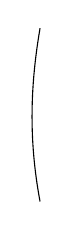
\begin{tikzpicture}\draw (0,0).. controls (-.15,.8) and (-.12,1.5)..(0,2.2);\end{tikzpicture}}
l'un des 2 $\beta_i$ :
\[
\begin{aligned}
&\tau_0\longrightarrow1\\
&\left\{\begin{aligned}\tau_i&\longrightarrow0\qquad i\ne0\\
\xi_j&\longrightarrow0\qquad j>0\end{aligned}\right.
\end{aligned}
\]
Conclusion \quad $H_*(K(\mathbb F_p,n),\mathbb Z)={}$ \deleted{l'autre} l'alg à puiss div libre eng par la partie d'exces $<n$ de
$\left\{\underset{\substack{i>0\\j>0}}{\operatorname{Sym}(\xi_i)\otimes\Lambda(\tau_j)}\right\}$

$H_*(K(\mathbb Z,n),\deleted{\mathbb F_p}\mathbb Z)$ : $\beta_2$ :
$\left\{\begin{aligned}\tau_j&\longrightarrow\xi_j\\ \xi_j&\longrightarrow0\end{aligned}\right\}$.

$\beta_2$ agit sur $H_*(K(\mathbb F_p,n),\mathbb Z)\xrightarrow{\beta_2}H_*(K(\mathbb F_p,n),\mathbb Z)$

C'est une derivation (anti com) :
\[
\begin{aligned}\tau_j&\longrightarrow\xi_j\\ \xi_j&\longrightarrow0\end{aligned}
\]
\[
\operatorname{Im}\beta_2=\ker\beta_2=H_*(K(\mathbb Z,n),\mathbb Z)_{(p)} .
\]
\figure{\begin{tikzpicture}\draw (0,0)--(1.2,0);\end{tikzpicture}}
La conjugaison $c:A\longrightarrow A$\quad $:A_*\longrightarrow A_*$ est explicitée dans Steenrod

Elle transforme l'un des $\beta$ dans l'autre et transporte la sous algebre (partie stable de) :
\diagram{\begin{tikzcd}[column sep=small,row sep=small]
(*)& H_*(K(\mathbb Z,n),\mathbb F_p)\arrow[r,"\sim"]\arrow[d,phantom,"\rotatebox{90}{$\subset$}"]&
H_*(K(\mathbb F_p,n),\mathbb Z)\arrow[dl,bend left=15]\\
&H_*(K(\mathbb F_p,n),\mathbb F_p)=A_*&
\end{tikzcd}}
\mspage{372}
